\documentclass[../main.tex]{subfiles}
\graphicspath{{\subfix{../images/}}}
\begin{document}



\subsection{Ortogonální transformace}

$\mathbf{Q} \in \mathbb{R}^{3\times 3}$ ortogonální\\
$\mathbf{Q} = (q_{ij})$

$\mathbb{T} = (\tau_{i_1...i_n})$\\
$\tilde{\mathbb{T}} = (\tilde{\tau}_{i_1...i_n})$, kde $\tilde{\tau}_{i_1...i_n} = q_{i_1j_1}q_{i_2j_2}...q_{i_nj_n}\tau_{j_1...j_n}$ 

$\lceil \mathbb{T} \rceil_{\mathcal{X}} = \mathbb{T}, \lceil \mathbb{T} \rceil_{\mathcal{Y}} = \tilde{\mathbb{T}}$

$(\vec{y}_1 \vec{y}_2 \vec{y}_3) = (\vec{x}_1 \vec{x}_2 \vec{x}_3 ) \mathbf{Q}$

\subsection{Invarianty tenzoru}
\begin{definition}
    Mějme skalární funkci $\lambda: \mathbb{R}^{3\times 3} \mapsto \mathbb{R}$.
    Funkce $\lambda = \lambda(\mathbb{T})$ se nazývá invariant tenzoru $\mathbb{T}$, právě když
    $\lambda((\tau_{ij}) ) = \lambda((\tilde{\tau}_{ij}))$ pro každou transformaci $\mathbf{Q}$.
\end{definition}


\begin{example}
    Determinant $\mathbb{T}$ je invariant

    \begin{equation*}
        (\tilde{\tau}_{ij}) = q_{ik} q_{jl} \tau_{kl} = (\mathbf{Q}^T \mathbb{T} \mathbf{Q})_{ij}
    \end{equation*}

    Dále platí
    \begin{equation*}
        \mathbf{Q}^T = \mathbf{Q}^{-1} \implies \det \mathbf{Q}^T \det \mathbf{Q} = 1
    \end{equation*}

    Proto 
    \begin{equation*}
        \det(\tilde{\tau}_{ij}) = \det(\mathbf{Q}^T \mathbb{T} \mathbf{Q}) =\det \mathbf{Q}^T\det \mathbb{T} \det \mathbf{Q} = \mathbb{T} 
    \end{equation*}

    Z charakteristický polynomu lze získat další invarianty

    \begin{equation*}
    \mathcal{l}(t) = \det(\mathbb{T} - t \mathbb{I}) = \det (\mathbf{Q}^T (\mathbb{T} - t \mathbb{I}) \mathbf{Q}) = 
    \det (\mathbf{Q}^T \mathbb{T} \mathbf{Q}  - t \mathbb{I}) 
    \end{equation*}

    Celkem dostáváme hlavní invarianty $\mathbb{T}$:

    \begin{equation*}
        _\mathbb{T}I_1 = Tr \mathbb{T} = \tau_{ii}
    \end{equation*}

    \begin{equation*}
        _\mathbb{T}I_2 = \frac{1}{2}((Tr \mathbb{T})^2 - Tr (\mathbb{T}^2))
    \end{equation*}

    \begin{equation*}
        _\mathbb{T}I_3 = \det \mathbb{T}
    \end{equation*}


\end{example}

\begin{remark}
    $\mathbb{S} = (\sigma_{ij}), \mathbb{T} = (\tau_{ij})$

    $\mathbb{S} \odot \mathbb{T} = \sigma_{ij} \tau_{ij}$

    $(\mathbf{Q}^\mathbb{T} \mathbf{Q})_{kr} = q_{ik}q_{ir} = \delta_{kr}$

    \begin{equation*}
        \tilde{\sigma}_{ij} \tilde{\tau}_{ij} = q_{ik}q_{jl}\sigma_{kl} q_{ir}q_{js}\tau_{rs} = \delta_{kr} \delta_{ls}
        \sigma_{kl}\tau_{rs} = \sigma_{kl}\tau_{kl}
    \end{equation*}

    Konkrétně $\mathbb(S) = \mathbb{I}$
    \begin{equation*}
        \mathbb{I} \odot \mathbb{T} = \delta_{ij} \tau_{ij} = \tau_{ii} = Tr \mathbb{T}
    \end{equation*}
\end{remark}


\subsection{Diferenciální počet s vektory a tenzory}

\begin{equation*}
    \nabla = (\frac{\partial}{\partial x_1}, \frac{\partial}{\partial x_2}, \frac{\partial}{\partial x_3}) = (\partial_1, \partial_2, \partial_3) =  (\partial_i)^\mathbb{T}
\end{equation*}


Gradient skalární funkce $f$
\begin{equation*}
    \nabla f = (\partial_i f)^\mathbb{T}
\end{equation*}

Gradient vektorové funkce $\vec{f} = (f_j)$ je tenzor
\begin{equation*}
    \nabla \vec{f} = (\partial_i f_j)
\end{equation*}

Divergence vektorového pole
\begin{equation*}
    \nabla \cdot \vec{f} = \partial_i \partial_i 
\end{equation*}


Rotace vektorového pole 
\begin{equation*}
    \nabla\times\vec{f} = \text{rot} \vec{f} = \text{curl} \vec{f} = (\varepsilon_{ikl} \partial_k f_l)
\end{equation*}

\section{Kinematika tekutin}
\subsection{Zálkadní předpoklady}
Zkoumáme materiálové těleso 
\begin{definition}
    Materiálové tělese $V\subset \mathbb{R}^3$ se považuje za kontinuum, právě když pro každou podmnožinu $A\subset V$ platí,
    že pokud jeho trojrozměrná Lebesgueova míra (objem) $m_3(A) = 0 \implies M(A) = 0$, kde $M(A)$ je míra vyjadřující hmotnost A 
\end{definition}

\begin{definition}
    Nechť $\Psi$, resp. $\vec{\Psi}$ je míra, respektive "vektorová míra" $\vec{\Psi} = (\psi_1 \psi_2 \psi_3)^T$
    taková, že $\forall \vec{x} \in V$ existuje konečná limita 

    \begin{equation*}
        \vec{\Psi} (\vec{x}) = \lim_{R\rightarrow0^+} \frac{\vec{\Psi}(B_R (\vec{x}))}{M (B_R (\vec{x}))}
    \end{equation*}

    Potom $\Psi$ (resp. $\vec{\Psi}$) nazýváme skalární (resp. vektorovou) fyzikální veličinou a $\psi$, resp. $\vec{\psi}$ je příslušná specifická veličina (vztažené na jednotku hmotnosti)
\end{definition}

\begin{example}
    $\Psi$ ... tepelná kapacita V \\
    $\psi$ ... specifická tepelná kapacita $(c_p, c_v)$

    $\vec{\Psi} = \vec{P}$ ... hybnost tělesa V \\
    $\vec{\psi} = \vec{V}$ ... rychlost 
\end{example}

Předpokládáme, že existuje $\forall \vec{x} \in V$
\begin{equation*}
    \varrho(\vec{x})= \lim_{R\rightarrow0^+} \frac{M(B_R (\vec{x}))}{m_3 (B_R (\vec{x}))} = \lim_{R\rightarrow0^+} \frac{M(B_R (\vec{x}))}{\frac{4}{3}\pi R^3} 
\end{equation*}
, což je hmotnostní hustota materiálu v bodě $\vec{x}$







\subsection{Referenční a aktuální konfigurace mat. tělesa}
Nechť v čase $t=0$ materiálové těleso zaujímá objem $V_0\subset \mathbb{R}^3$ a dojde k 
vývoji tak, že v čase $t>0$ těleso zaujme objem $V(t)$, tj $V(0) = V_{0}$

\begin{center}
    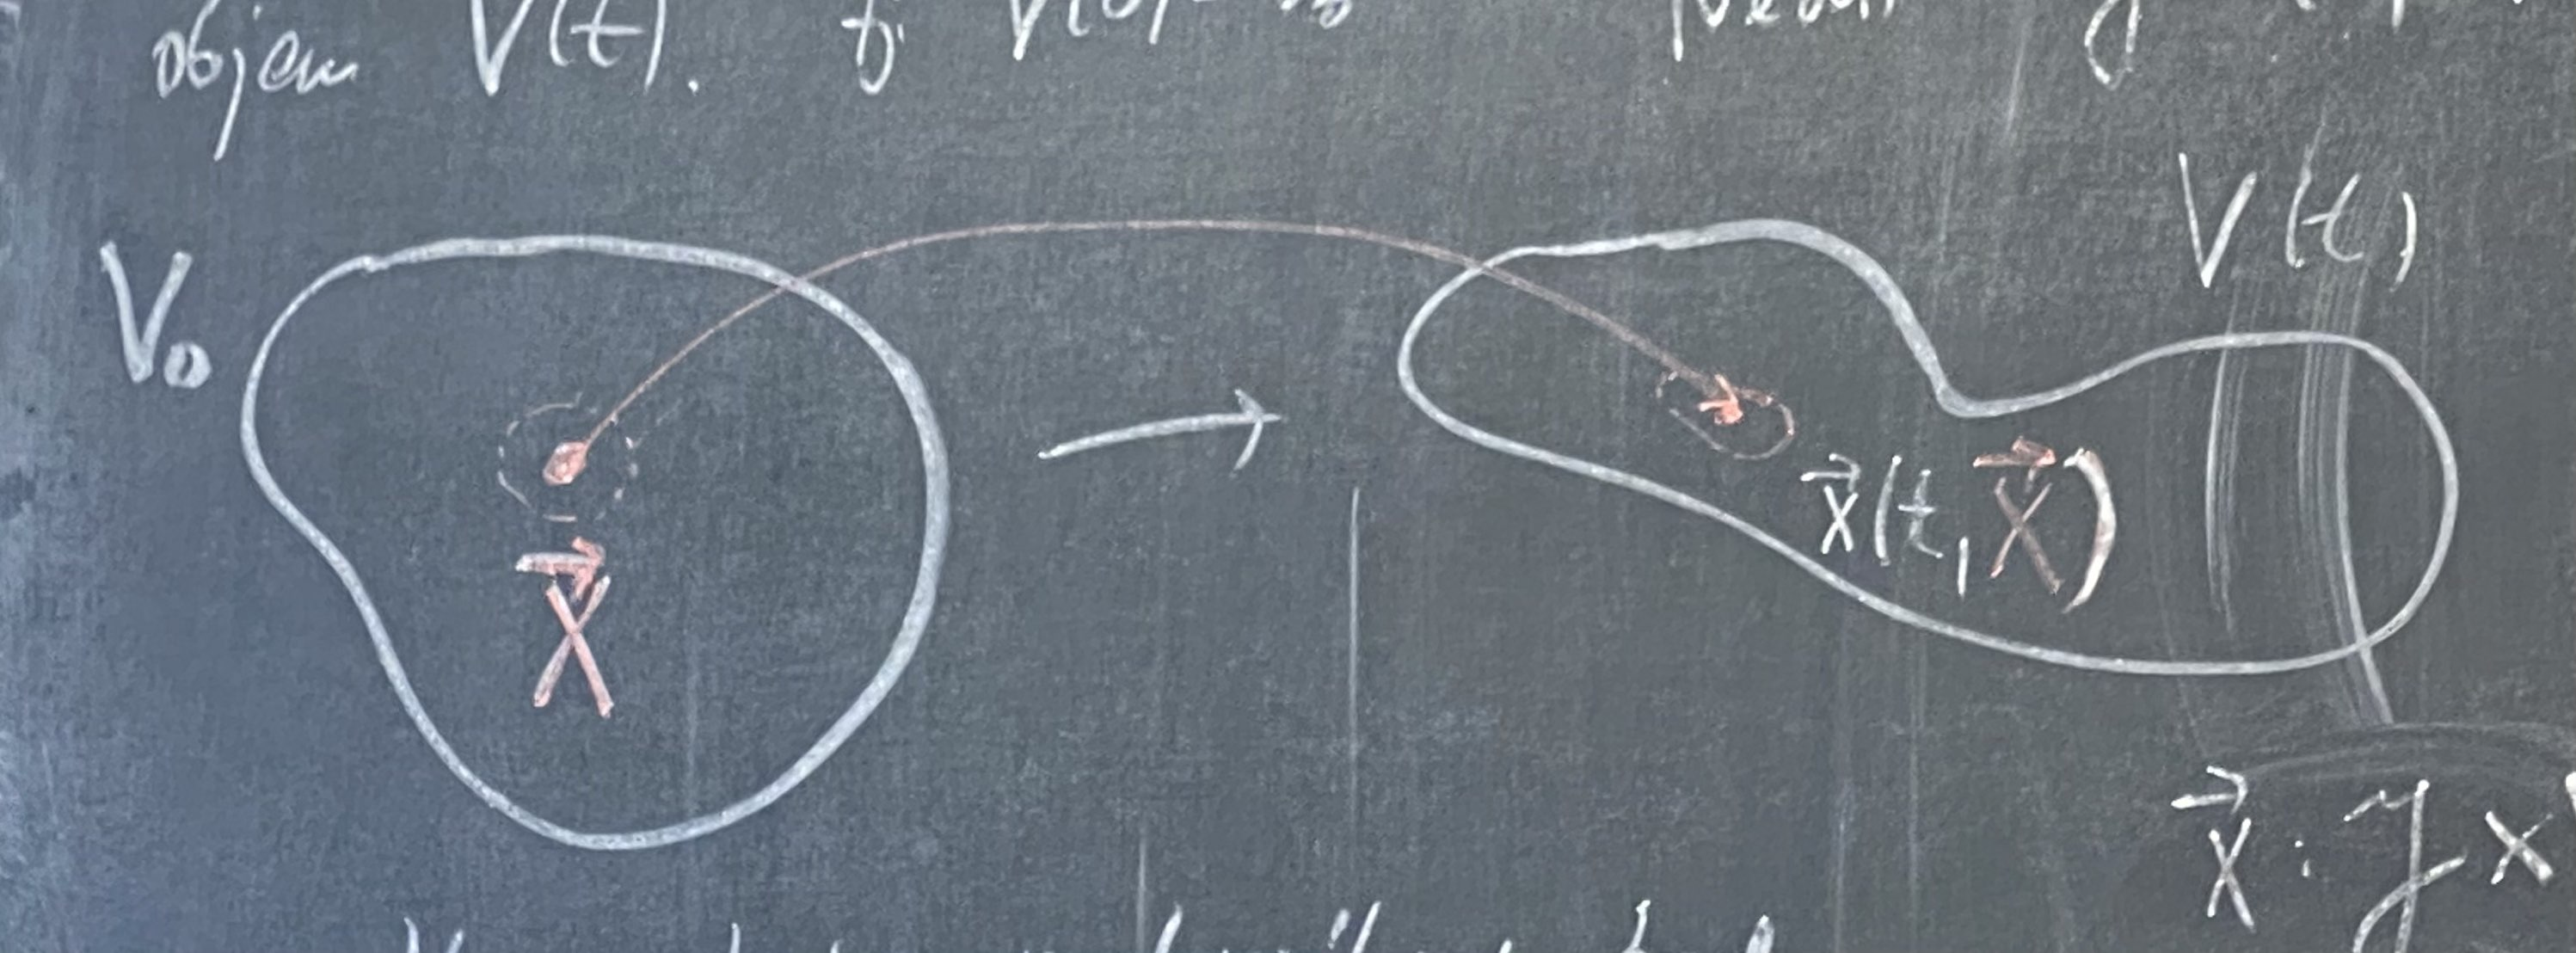
\includegraphics[width=0.5\linewidth]{images/13-10-konfigurace.jpg}
\end{center}
prvky $V_0$ nazýváme materiálové body a značíme $\vec{X} \in V_0 $.\\
Nechť $\mathcal{y} = (0, t_{max})$ je časový interval.

$\vec{x} : \mathcal{y} \times V_0 \mapsto \mathbb{R}^3$\\
$\vec{x}(t, \vec{X})$ udává pozici bodu $\vec{X}$ v čase $t$.

$\vec{x}$ je prosté a regulární, tj $\det\frac{\partial x_i}{\partial X_j} \neq 0$

Z tohoto faktu víme, že existuje inverzní zobrazení $\vec{X} : \mathcal{y} \times \mathbb{R}^3 \mapsto V_0$  a 
$\vec{X}(t, \vec{x})$ určuje "který" materiálový bod se v čase $t$ nachází na pozici $\vec{x}$.

$\vec{X}$ identifikuje materiálové body dle jejich pozice v čase 0, takzvané materiálové souřadnice\\
$\vec{x}$ nazveme aktuální (prostorové souřadnice)



Nechť je dána skalární intenzivní (např. specifická) veličina, jejíž hodnotu vyjádříme funkcí $w=w(t, \vec{X})$
respektive funkcí $W = W(t, \vec{x})$.\\
Platí mezi nimi následující vztah (nazvěme ho jako základní rovnost)
\begin{equation*}
    w(t,\vec{X}) = W(t, \vec{x}), \text{kde } \vec{x} = \vec{x}(t, \vec{X})  
\end{equation*} 
neboli $w(t, \vec{X}) = W(t, \vec{x}(t, \vec{X}))$




\subsection{Materiálová derivace}

\begin{align*}
    \frac{\partial w}{\partial t} (t, \vec{X}) &= \frac{\partial}{\partial t} \left[ W(t, \vec{x}(t, \vec{X}))  \right]_(t, \vec{X})\\
    &= \frac{\partial W}{\partial t}\mid_{(t, \vec{x}(t, \vec{X}))}1  + \frac{\partial W}{\partial x_k}\mid_{(t, \vec{x}(t, \vec{X}))} \cdot \frac{\partial x_k}{\partial t} \mid_{(t,\vec{X})}\\
    &= \left(  \frac{\partial W}{\partial t} + \vec{V} \cdot \nabla W                     \right)\mid_{(t, \vec{x}(t, \vec{X}))}
\end{align*}

Definujeme $\frac{D}{D t} = \frac{\partial}{ \partial t} + \vec{V} \cdot \nabla$ jako operátor materiálové derivace.\\
Poté předchozí vztah přepíšeme jako $\frac{\partial w}{\partial t} (t, \vec{X}) = \frac{D W}{D t} (t, \vec{x})$

\begin{example}
    Zrychlení materiálového bodu $\vec{X}$ je 
    \begin{equation*}
        \vec{a}(t, \vec{X}) = \frac{\partial \vec{v}}{\partial t} (t, \vec{X}) = \frac{D \vec{V}}{D t} (t, \vec{x}), \text{kde } \vec{x} = \vec{x}(t, \vec{X})
    \end{equation*}
\end{example}

\end{document}